\documentclass[]{article}
\usepackage{lmodern}
\usepackage{amssymb,amsmath}
\usepackage{ifxetex,ifluatex}
\usepackage{fixltx2e} % provides \textsubscript
\ifnum 0\ifxetex 1\fi\ifluatex 1\fi=0 % if pdftex
  \usepackage[T1]{fontenc}
  \usepackage[utf8]{inputenc}
\else % if luatex or xelatex
  \ifxetex
    \usepackage{mathspec}
  \else
    \usepackage{fontspec}
  \fi
  \defaultfontfeatures{Ligatures=TeX,Scale=MatchLowercase}
\fi
% use upquote if available, for straight quotes in verbatim environments
\IfFileExists{upquote.sty}{\usepackage{upquote}}{}
% use microtype if available
\IfFileExists{microtype.sty}{%
\usepackage{microtype}
\UseMicrotypeSet[protrusion]{basicmath} % disable protrusion for tt fonts
}{}
\usepackage[margin=1in]{geometry}
\usepackage{hyperref}
\hypersetup{unicode=true,
            pdftitle={Exploratory Data Analysis on the CO\_County\_x\_2014\_2018.xlxs},
            pdfauthor={David Martinez (davelovesdata@gmail.com)},
            pdfborder={0 0 0},
            breaklinks=true}
\urlstyle{same}  % don't use monospace font for urls
\usepackage{color}
\usepackage{fancyvrb}
\newcommand{\VerbBar}{|}
\newcommand{\VERB}{\Verb[commandchars=\\\{\}]}
\DefineVerbatimEnvironment{Highlighting}{Verbatim}{commandchars=\\\{\}}
% Add ',fontsize=\small' for more characters per line
\usepackage{framed}
\definecolor{shadecolor}{RGB}{248,248,248}
\newenvironment{Shaded}{\begin{snugshade}}{\end{snugshade}}
\newcommand{\AlertTok}[1]{\textcolor[rgb]{0.94,0.16,0.16}{#1}}
\newcommand{\AnnotationTok}[1]{\textcolor[rgb]{0.56,0.35,0.01}{\textbf{\textit{#1}}}}
\newcommand{\AttributeTok}[1]{\textcolor[rgb]{0.77,0.63,0.00}{#1}}
\newcommand{\BaseNTok}[1]{\textcolor[rgb]{0.00,0.00,0.81}{#1}}
\newcommand{\BuiltInTok}[1]{#1}
\newcommand{\CharTok}[1]{\textcolor[rgb]{0.31,0.60,0.02}{#1}}
\newcommand{\CommentTok}[1]{\textcolor[rgb]{0.56,0.35,0.01}{\textit{#1}}}
\newcommand{\CommentVarTok}[1]{\textcolor[rgb]{0.56,0.35,0.01}{\textbf{\textit{#1}}}}
\newcommand{\ConstantTok}[1]{\textcolor[rgb]{0.00,0.00,0.00}{#1}}
\newcommand{\ControlFlowTok}[1]{\textcolor[rgb]{0.13,0.29,0.53}{\textbf{#1}}}
\newcommand{\DataTypeTok}[1]{\textcolor[rgb]{0.13,0.29,0.53}{#1}}
\newcommand{\DecValTok}[1]{\textcolor[rgb]{0.00,0.00,0.81}{#1}}
\newcommand{\DocumentationTok}[1]{\textcolor[rgb]{0.56,0.35,0.01}{\textbf{\textit{#1}}}}
\newcommand{\ErrorTok}[1]{\textcolor[rgb]{0.64,0.00,0.00}{\textbf{#1}}}
\newcommand{\ExtensionTok}[1]{#1}
\newcommand{\FloatTok}[1]{\textcolor[rgb]{0.00,0.00,0.81}{#1}}
\newcommand{\FunctionTok}[1]{\textcolor[rgb]{0.00,0.00,0.00}{#1}}
\newcommand{\ImportTok}[1]{#1}
\newcommand{\InformationTok}[1]{\textcolor[rgb]{0.56,0.35,0.01}{\textbf{\textit{#1}}}}
\newcommand{\KeywordTok}[1]{\textcolor[rgb]{0.13,0.29,0.53}{\textbf{#1}}}
\newcommand{\NormalTok}[1]{#1}
\newcommand{\OperatorTok}[1]{\textcolor[rgb]{0.81,0.36,0.00}{\textbf{#1}}}
\newcommand{\OtherTok}[1]{\textcolor[rgb]{0.56,0.35,0.01}{#1}}
\newcommand{\PreprocessorTok}[1]{\textcolor[rgb]{0.56,0.35,0.01}{\textit{#1}}}
\newcommand{\RegionMarkerTok}[1]{#1}
\newcommand{\SpecialCharTok}[1]{\textcolor[rgb]{0.00,0.00,0.00}{#1}}
\newcommand{\SpecialStringTok}[1]{\textcolor[rgb]{0.31,0.60,0.02}{#1}}
\newcommand{\StringTok}[1]{\textcolor[rgb]{0.31,0.60,0.02}{#1}}
\newcommand{\VariableTok}[1]{\textcolor[rgb]{0.00,0.00,0.00}{#1}}
\newcommand{\VerbatimStringTok}[1]{\textcolor[rgb]{0.31,0.60,0.02}{#1}}
\newcommand{\WarningTok}[1]{\textcolor[rgb]{0.56,0.35,0.01}{\textbf{\textit{#1}}}}
\usepackage{graphicx,grffile}
\makeatletter
\def\maxwidth{\ifdim\Gin@nat@width>\linewidth\linewidth\else\Gin@nat@width\fi}
\def\maxheight{\ifdim\Gin@nat@height>\textheight\textheight\else\Gin@nat@height\fi}
\makeatother
% Scale images if necessary, so that they will not overflow the page
% margins by default, and it is still possible to overwrite the defaults
% using explicit options in \includegraphics[width, height, ...]{}
\setkeys{Gin}{width=\maxwidth,height=\maxheight,keepaspectratio}
\IfFileExists{parskip.sty}{%
\usepackage{parskip}
}{% else
\setlength{\parindent}{0pt}
\setlength{\parskip}{6pt plus 2pt minus 1pt}
}
\setlength{\emergencystretch}{3em}  % prevent overfull lines
\providecommand{\tightlist}{%
  \setlength{\itemsep}{0pt}\setlength{\parskip}{0pt}}
\setcounter{secnumdepth}{0}
% Redefines (sub)paragraphs to behave more like sections
\ifx\paragraph\undefined\else
\let\oldparagraph\paragraph
\renewcommand{\paragraph}[1]{\oldparagraph{#1}\mbox{}}
\fi
\ifx\subparagraph\undefined\else
\let\oldsubparagraph\subparagraph
\renewcommand{\subparagraph}[1]{\oldsubparagraph{#1}\mbox{}}
\fi

%%% Use protect on footnotes to avoid problems with footnotes in titles
\let\rmarkdownfootnote\footnote%
\def\footnote{\protect\rmarkdownfootnote}

%%% Change title format to be more compact
\usepackage{titling}

% Create subtitle command for use in maketitle
\providecommand{\subtitle}[1]{
  \posttitle{
    \begin{center}\large#1\end{center}
    }
}

\setlength{\droptitle}{-2em}

  \title{Exploratory Data Analysis on the CO\_County\_x\_2014\_2018.xlxs}
    \pretitle{\vspace{\droptitle}\centering\huge}
  \posttitle{\par}
    \author{David Martinez
(\href{mailto:davelovesdata@gmail.com}{\nolinkurl{davelovesdata@gmail.com}})}
    \preauthor{\centering\large\emph}
  \postauthor{\par}
      \predate{\centering\large\emph}
  \postdate{\par}
    \date{May 7, 2019}


\begin{document}
\maketitle

\hypertarget{purpose}{%
\subsection{Purpose}\label{purpose}}

To perform Exploratory Data Analysis on a dataset containing four years
of Colorado county level medical and recreational marijuana sales as
well as state revenue (taxes) collected. Two excel workbook sheets are
imported to R and merged together, one for sales, the other for taxes.

\hypertarget{sales-file-description-co_county_sales_2014_2018.xlsx}{%
\paragraph{\texorpdfstring{1. Sales file description
(CO\_County\_Sales\_2014\_2018.xlsx)}{1. Sales file description (CO\_County\_Sales\_2014\_2018.xlsx) }}\label{sales-file-description-co_county_sales_2014_2018.xlsx}}

The sales files contains not only county level medical and recreational
sales by year, but also population information and location information
(State, County, Latitude, Longitude, Region). Additionally, medical and
recreational sales for each county were applied against county
population to determine an average of sales per county citizen for both
medical and recreational sales.

\textbf{Dataset fields:} State - Currently only ``COLORADO'' County -
Colorado County Name (e.g., ``Adams'' or ``Yuma'') Latitude - Latitude
of County center Longitude - Longitude of County Center Region - An
arbitrary assignment I made to quarter the state into geographic
quadrants. Year - Collection Year Population - Estimated population
between census reporting periods Med\_Sales - County level sales of
Medical Marijuana (see value explanation below) Rec\_Sales - County
level sales of Recreational Marijuana (see value explanation below)
med\_sales\_per\_citizen - a calculated value determined by dividing the
``Med\_Sales'' value by the ``Population'' value.
rec\_sales\_pre\_citizen - a calculated value determined by dividing the
``Rec\_Sales'' value by the ``Population'' value.

Med\_Sales, Rec\_sales, and the two calculated values have three
possible values: \textbf{0} = No Sales of legal Marijuana occurred in
that county. The original source material did not include counties that
had no sales. This information was added to show a full statewide
picture as well as county adoption over time. \textbf{NR} = Not
releasable due to confidentiality requirements. The sum of all NR
counties (``Not Reported'' in the `County' column) are captured as the
last line for each year. \textbf{x} = A positive number representing
sales at the dollar level.

\hypertarget{taxes-file-description-co_county_taxes_2014_2018.xlsx}{%
\paragraph{\texorpdfstring{2. Taxes file description
(CO\_County\_Taxes\_2014\_2018.xlsx)}{2. Taxes file description (CO\_County\_Taxes\_2014\_2018.xlsx) }}\label{taxes-file-description-co_county_taxes_2014_2018.xlsx}}

The taxes file contains taxes collected per county in three columns:
Medical Sales Tax (2.9\%), Retail Sales Tax (2.9\%), Retail Marijuana
Special Sales Tax.

\textbf{Dataset fields:} County - Colorado County Name (e.g., ``Adams''
or ``Yuma'') Year - Collection Year Medical Sales Tax (2.9\%) - Sales
tax applied to medical marijuana only. This is the only state tax paid.
Retail Sales Tax (2.9\%) - Sales tax applied to retail marijuana.
Starting in 2018, this tax was no longer collected. Retail Marijuana
Special Sales Tax - an additional tax on retail marijuana sales.

Medical Sales Tax (2.9\%), Retail Sales Tax (2.9\%), Retail Marijuana
Special Sales Tax have three possible values: \textbf{0} = No taxes from
legal Marijuana occurred in that county. The original source material
did not include counties that had no tax information. This information
was added to show a full statewide picture as well as county adoption
over time. \textbf{NR} = Not releasable due to confidentiality
requirements. The sum of all NR counties (``Not Reported'' in the
`County' column) are captured as the last line for each year. \textbf{x}
= A number representing taxes at the dollar level. Negative values
indicate previous months overpayment of taxes being returned.

\hypertarget{data-collection-and-merging-steps}{%
\subsection{Data Collection and Merging
steps}\label{data-collection-and-merging-steps}}

\hypertarget{dependencies}{%
\subsubsection{Dependencies}\label{dependencies}}

If needed, these packages can be installed using the install.packages()
function

\begin{Shaded}
\begin{Highlighting}[]
\KeywordTok{library}\NormalTok{(}\StringTok{"readxl"}\NormalTok{)}
\KeywordTok{library}\NormalTok{(}\StringTok{"formattable"}\NormalTok{)}
\KeywordTok{library}\NormalTok{(}\StringTok{"tidyverse"}\NormalTok{)}
\KeywordTok{library}\NormalTok{(}\StringTok{"tidyr"}\NormalTok{)}
\KeywordTok{library}\NormalTok{(}\StringTok{"ggplot2"}\NormalTok{)}
\KeywordTok{library}\NormalTok{(}\StringTok{"ggrepel"}\NormalTok{)}
\end{Highlighting}
\end{Shaded}

\hypertarget{collect-and-merge-data}{%
\subsubsection{Collect and Merge data}\label{collect-and-merge-data}}

The two files are read into tibbles and then merged into a dataframe.
Data is subsetted to remove 2018 values. A loop is performed to convert
the sales and tax features to numeric and currency.

\begin{Shaded}
\begin{Highlighting}[]
\CommentTok{#gather sales and tax data into tibbles}
\NormalTok{sales_mj <-}\StringTok{ }\KeywordTok{read_xlsx}\NormalTok{(}\StringTok{"CO_County_Sales_2014_2018.xlsx"}\NormalTok{, }\DataTypeTok{sheet =} \StringTok{"aggregate"}\NormalTok{, }\DataTypeTok{range =} \OtherTok{NULL}\NormalTok{, }\DataTypeTok{col_names =} \OtherTok{TRUE}\NormalTok{)}
\NormalTok{taxes_mj <-}\StringTok{ }\KeywordTok{read_xlsx}\NormalTok{(}\StringTok{"CO_County_Taxes_2014_2018.xlsx"}\NormalTok{, }\DataTypeTok{sheet =} \StringTok{"aggregate"}\NormalTok{, }\DataTypeTok{range =} \OtherTok{NULL}\NormalTok{, }\DataTypeTok{col_names =} \OtherTok{TRUE}\NormalTok{)}

\CommentTok{#merge the two tibbles - \{base\} merge returns a dataframe}
\NormalTok{CCMDs <-}\StringTok{ }\KeywordTok{merge}\NormalTok{(sales_mj, taxes_mj)}

\CommentTok{#remove 2018 values until both spreadsheets are fully populated}
\NormalTok{CCMDs <-}\StringTok{ }\KeywordTok{subset}\NormalTok{(CCMDs, Year }\OperatorTok{<}\StringTok{ "2018"}\NormalTok{)}

\CommentTok{#create a list of column names for columns 8 through 14 - these are the columns related to sales and taxes}
\NormalTok{cashcol <-}\StringTok{ }\KeywordTok{colnames}\NormalTok{(CCMDs[}\DecValTok{8}\OperatorTok{:}\DecValTok{14}\NormalTok{])}

\CommentTok{#loop to convert sales/tax columns to numeric/currency - this will introduce NAs for each of the 7 columns (resulting in a warning for each column)}
\ControlFlowTok{for}\NormalTok{ (i }\ControlFlowTok{in}\NormalTok{ cashcol) \{}
\NormalTok{  CCMDs[[i]] <-}\StringTok{ }\KeywordTok{as.numeric}\NormalTok{(CCMDs[[i]])   }\CommentTok{#character to numeric}
\NormalTok{  CCMDs[[i]] <-}\StringTok{ }\KeywordTok{currency}\NormalTok{(CCMDs[[i]], }\DataTypeTok{digits =}\NormalTok{ 0L) }\CommentTok{#numeric but with currency symbology}
\NormalTok{\}}
\end{Highlighting}
\end{Shaded}

\begin{verbatim}
## Warning: NAs introduced by coercion

## Warning: NAs introduced by coercion

## Warning: NAs introduced by coercion

## Warning: NAs introduced by coercion

## Warning: NAs introduced by coercion

## Warning: NAs introduced by coercion

## Warning: NAs introduced by coercion
\end{verbatim}

\begin{Shaded}
\begin{Highlighting}[]
\CommentTok{#clean up unneeded files}
\KeywordTok{rm}\NormalTok{(cashcol, i)}
\KeywordTok{rm}\NormalTok{(sales_mj, taxes_mj)}

\CommentTok{#write dataframe to disk}
\KeywordTok{write_excel_csv}\NormalTok{(CCMDs, }\StringTok{"CCMDs.csv"}\NormalTok{, }\DataTypeTok{na =} \StringTok{"NA"}\NormalTok{, }\DataTypeTok{append =} \OtherTok{FALSE}\NormalTok{)}
\end{Highlighting}
\end{Shaded}

\hypertarget{exploratory-data-analysis}{%
\subsection{Exploratory Data Analysis}\label{exploratory-data-analysis}}

\begin{Shaded}
\begin{Highlighting}[]
\KeywordTok{summary}\NormalTok{(CCMDs)}
\end{Highlighting}
\end{Shaded}

\begin{verbatim}
##     County               Year         State              Latitude    
##  Length:260         Min.   :2014   Length:260         Min.   :37.20  
##  Class :character   1st Qu.:2015   Class :character   1st Qu.:38.01  
##  Mode  :character   Median :2016   Mode  :character   Median :39.07  
##                     Mean   :2016                      Mean   :38.98  
##                     3rd Qu.:2016                      3rd Qu.:39.86  
##                     Max.   :2017                      Max.   :40.87  
##                                                       NA's   :4      
##    Longitude         Region            Population       Med_Sales        
##  Min.   :-108.6   Length:260         Min.   :   689   Min.   :        0  
##  1st Qu.:-106.9   Class :character   1st Qu.:  5719   1st Qu.:        0  
##  Median :-105.5   Mode  :character   Median : 14366   Median :        0  
##  Mean   :-105.4                      Mean   : 85681   Mean   :  8349120  
##  3rd Qu.:-103.8                      3rd Qu.: 42846   3rd Qu.:  2726766  
##  Max.   :-102.3                      Max.   :705651   Max.   :210860875  
##  NA's   :4                           NA's   :4        NA's   :61         
##    Rec_Sales         med_sales_per_citizen rec_sales_per_citizen
##  Min.   :        0   Min.   :  0.00        Min.   :   0.0       
##  1st Qu.:        0   1st Qu.:  0.00        1st Qu.:   0.0       
##  Median :        0   Median :  0.00        Median :   0.0       
##  Mean   : 12479031   Mean   : 32.53        Mean   : 149.6       
##  3rd Qu.:  7869992   3rd Qu.: 43.52        3rd Qu.: 206.1       
##  Max.   :374673239   Max.   :909.01        Max.   :3093.2       
##  NA's   :34          NA's   :65            NA's   :38           
##  Medical Sales Tax (2.9%) Retail Sales Tax (2.9%)
##  Min.   :      0          Min.   :      0        
##  1st Qu.:      0          1st Qu.:      0        
##  Median :      0          Median :      0        
##  Mean   : 230108          Mean   : 289108        
##  3rd Qu.:  81149          3rd Qu.: 188086        
##  Max.   :6011329          Max.   :8092488        
##  NA's   :62               NA's   :36             
##  Retail Marijuana Special Sales Tax
##  Min.   :       0                  
##  1st Qu.:       0                  
##  Median :       0                  
##  Mean   : 1135213                  
##  3rd Qu.:  659683                  
##  Max.   :39493849                  
##  NA's   :34
\end{verbatim}

There are 260 observation with 14 variables. There are 346 NA's
(\textasciitilde{}10\%) that will need to be addressed.

\begin{Shaded}
\begin{Highlighting}[]
\CommentTok{#count the NAs}
\KeywordTok{sum}\NormalTok{(}\KeywordTok{is.na}\NormalTok{(CCMDs))}
\end{Highlighting}
\end{Shaded}

\begin{verbatim}
## [1] 346
\end{verbatim}

\begin{Shaded}
\begin{Highlighting}[]
\CommentTok{#remove the NAs}
\NormalTok{CCMDs <-}\StringTok{ }\KeywordTok{na.omit}\NormalTok{(CCMDs)}

\KeywordTok{plot}\NormalTok{(CCMDs[,}\DecValTok{7}\OperatorTok{:}\DecValTok{14}\NormalTok{])}
\end{Highlighting}
\end{Shaded}

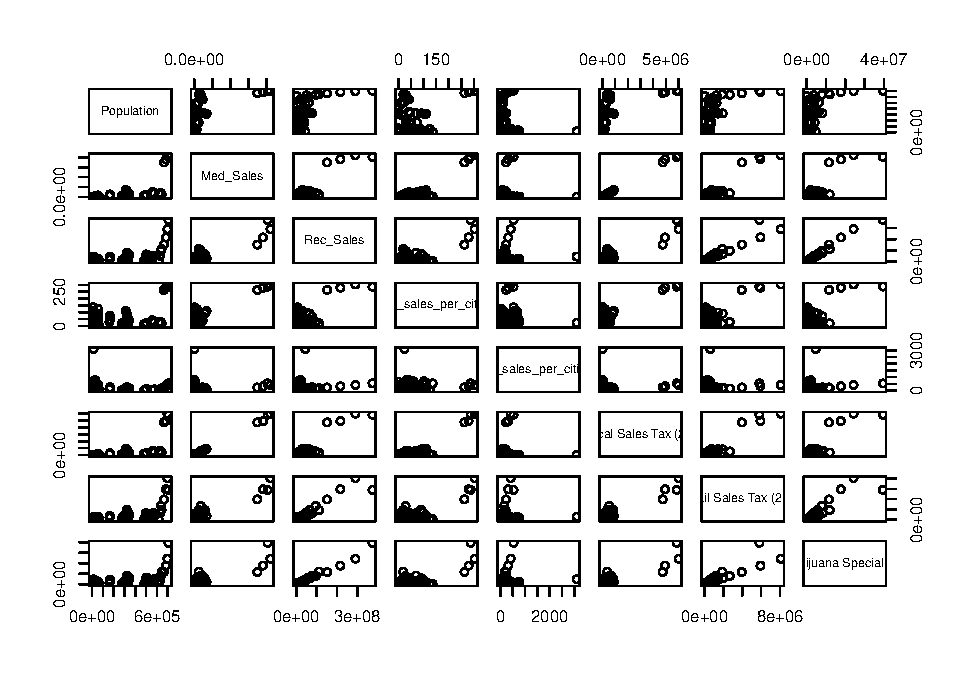
\includegraphics{01-Build_DS_and_EDA_files/figure-latex/unnamed-chunk-4-1.pdf}
Right from the start, the data are redundant. Specifically, the
`med\_sales\_per\_citizen' and `rec\_sales\_per\_citizen' variables
which are calculated by dividing the county sales by the county
population. Similarly, the tax data is also a function of the sales
data. For now, I'm going to ignore that data.

\begin{Shaded}
\begin{Highlighting}[]
\KeywordTok{library}\NormalTok{(corrplot)}
\end{Highlighting}
\end{Shaded}

\begin{verbatim}
## corrplot 0.84 loaded
\end{verbatim}

\begin{Shaded}
\begin{Highlighting}[]
\CommentTok{#subset out unnecessary columns}
\KeywordTok{plot}\NormalTok{(CCMDs[,}\DecValTok{7}\OperatorTok{:}\DecValTok{9}\NormalTok{])}
\end{Highlighting}
\end{Shaded}

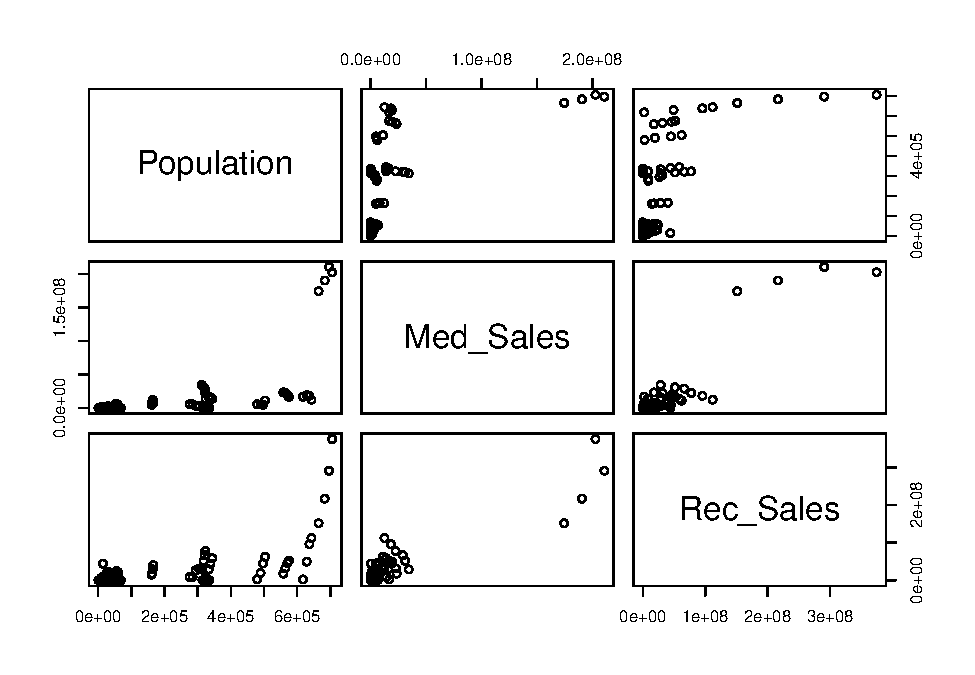
\includegraphics{01-Build_DS_and_EDA_files/figure-latex/unnamed-chunk-5-1.pdf}

\begin{Shaded}
\begin{Highlighting}[]
\CommentTok{#corrplot the value features}
\NormalTok{m <-}\StringTok{ }\KeywordTok{cor}\NormalTok{(CCMDs[, }\KeywordTok{c}\NormalTok{(}\DecValTok{7}\OperatorTok{:}\DecValTok{9}\NormalTok{)], }\DataTypeTok{use =} \StringTok{"complete.obs"}\NormalTok{, }\DataTypeTok{method =} \StringTok{"spearman"}\NormalTok{)}
\KeywordTok{corrplot}\NormalTok{(m, }\DataTypeTok{method=}\StringTok{"number"}\NormalTok{, }\DataTypeTok{type =} \StringTok{"lower"}\NormalTok{, }\DataTypeTok{order =} \StringTok{"hclust"}\NormalTok{, }\DataTypeTok{tl.srt =} \DecValTok{45}\NormalTok{)}
\end{Highlighting}
\end{Shaded}

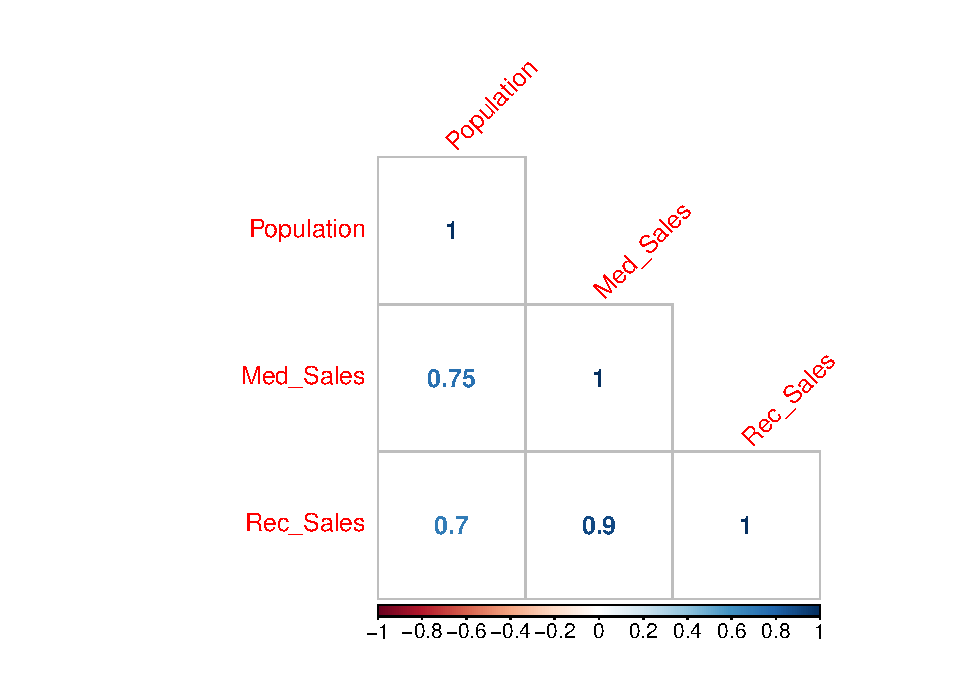
\includegraphics{01-Build_DS_and_EDA_files/figure-latex/unnamed-chunk-5-2.pdf}
Of course, it makes sense that population would correlate to sales and
that med/rec sales would correlate so highly to each other.

\begin{Shaded}
\begin{Highlighting}[]
\CommentTok{#disable scientific notation}
\KeywordTok{options}\NormalTok{(}\DataTypeTok{scipen =} \DecValTok{999}\NormalTok{)}

\CommentTok{#table(CCMDs[, 1,8:9])}

\CommentTok{#filter by year}

\KeywordTok{ggplot}\NormalTok{(}\DataTypeTok{data=}\NormalTok{CCMDs, }\KeywordTok{aes}\NormalTok{(}\DataTypeTok{x =}\NormalTok{ Population))}\OperatorTok{+}
\StringTok{  }\KeywordTok{geom_point}\NormalTok{(}\KeywordTok{aes}\NormalTok{(}\DataTypeTok{y =}\NormalTok{ Rec_Sales}\OperatorTok{/}\DecValTok{100000}\NormalTok{), }\DataTypeTok{color=}\StringTok{"green"}\NormalTok{, }\DataTypeTok{show.legend =} \OtherTok{TRUE}\NormalTok{, }\DataTypeTok{size =} \FloatTok{1.25}\NormalTok{)}\OperatorTok{+}
\StringTok{  }\KeywordTok{geom_point}\NormalTok{(}\KeywordTok{aes}\NormalTok{(}\DataTypeTok{y =}\NormalTok{ Med_Sales}\OperatorTok{/}\DecValTok{100000}\NormalTok{), }\DataTypeTok{color=}\StringTok{"red"}\NormalTok{, }\DataTypeTok{show.legend =} \OtherTok{TRUE}\NormalTok{, }\DataTypeTok{size =} \FloatTok{1.25}\NormalTok{)}\OperatorTok{+}
\StringTok{  }\KeywordTok{labs}\NormalTok{(}\DataTypeTok{title=}\StringTok{"Medical and Retail Marijuana Sales as a measure of population"}\NormalTok{, }\DataTypeTok{x=} \StringTok{"Colorado County Population"}\NormalTok{, }\DataTypeTok{y=} \StringTok{"Marijuana Sales per $100K"}\NormalTok{)}\OperatorTok{+}
\StringTok{  }\KeywordTok{theme_bw}\NormalTok{()}\OperatorTok{+}
\StringTok{  }\KeywordTok{coord_flip}\NormalTok{()}
\end{Highlighting}
\end{Shaded}

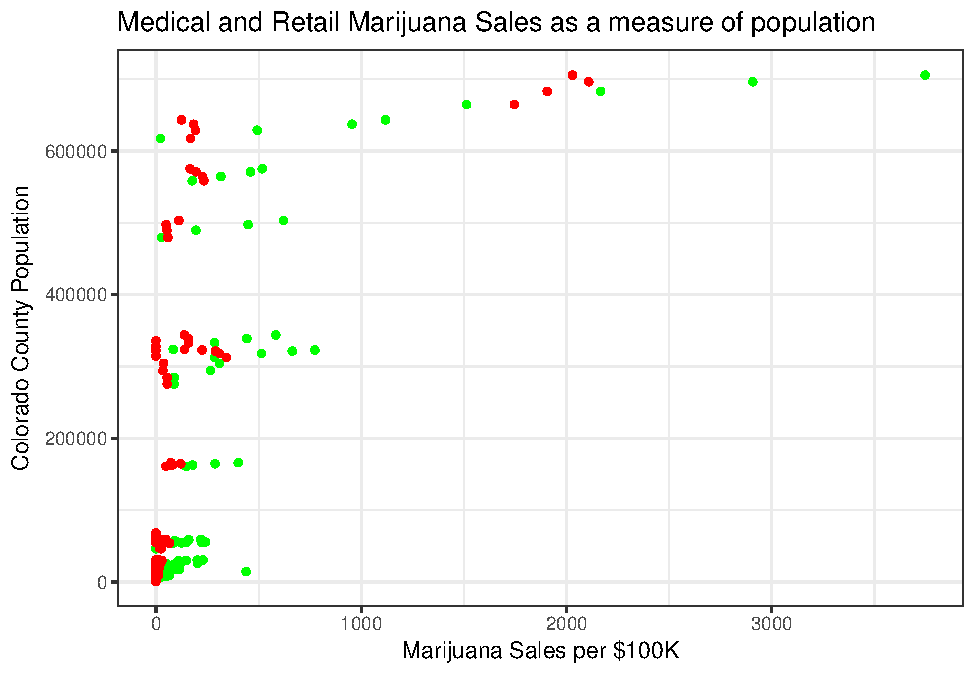
\includegraphics{01-Build_DS_and_EDA_files/figure-latex/unnamed-chunk-6-1.pdf}
Four clusters seem to be immediately evident (low pop/low sales, med
pop/low sales, high pop/low sales, and high pop/higher sales starting
around 1000K). Cluster analysis will need to be performed to validate
optimal cluster size and groupings.

\begin{Shaded}
\begin{Highlighting}[]
\CommentTok{#first scale and sequester the data fields of interest into a matrix. }
\NormalTok{CCMDs_scale <-}\StringTok{ }\KeywordTok{scale}\NormalTok{(CCMDs[,}\DecValTok{7}\OperatorTok{:}\DecValTok{9}\NormalTok{])}

\CommentTok{#use elbow method to determine optimal number of clusters}
\KeywordTok{set.seed}\NormalTok{(}\DecValTok{12345}\NormalTok{)}

\NormalTok{k.max <-}\StringTok{ }\DecValTok{15}
\NormalTok{data <-}\StringTok{ }\NormalTok{CCMDs_scale}

\NormalTok{wss <-}\StringTok{ }\KeywordTok{sapply}\NormalTok{(}\DecValTok{1}\OperatorTok{:}\NormalTok{k.max, }\ControlFlowTok{function}\NormalTok{(k)\{}\KeywordTok{kmeans}\NormalTok{(data, k, }\DataTypeTok{nstart=}\DecValTok{50}\NormalTok{, }\DataTypeTok{iter.max=}\DecValTok{15}\NormalTok{)}\OperatorTok{$}\NormalTok{tot.withinss\})}

\CommentTok{#generate elbow plot}
\KeywordTok{plot}\NormalTok{(}\DecValTok{1}\OperatorTok{:}\NormalTok{k.max, wss, }\DataTypeTok{type=}\StringTok{"b"}\NormalTok{, }\DataTypeTok{pch=}\DecValTok{19}\NormalTok{, }\DataTypeTok{frame=}\OtherTok{FALSE}\NormalTok{, }\DataTypeTok{xlab=}\StringTok{"number of clusters K"}\NormalTok{, }\DataTypeTok{ylab=}\StringTok{"Total within-clusters sum of squares"}\NormalTok{)}
\end{Highlighting}
\end{Shaded}

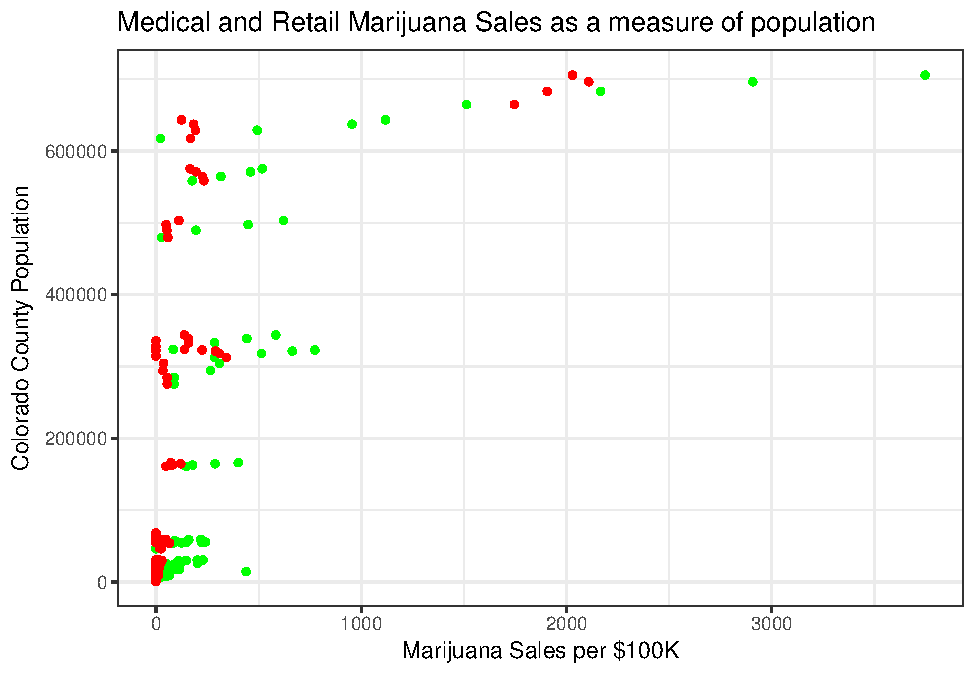
\includegraphics{01-Build_DS_and_EDA_files/figure-latex/unnamed-chunk-7-1.pdf}

\begin{Shaded}
\begin{Highlighting}[]
\CommentTok{#use kmeans to perform cluster identification}
\NormalTok{cluster <-}\StringTok{ }\KeywordTok{kmeans}\NormalTok{(CCMDs_scale, }\DataTypeTok{centers=}\DecValTok{3}\NormalTok{, }\DataTypeTok{iter.max=}\DecValTok{50}\NormalTok{, }\DataTypeTok{nstart=}\DecValTok{5}\NormalTok{)}

\CommentTok{#bind the cluster field to to the values from scale}
\NormalTok{cluster <-}\StringTok{ }\NormalTok{cluster}\OperatorTok{$}\NormalTok{cluster}

\CommentTok{#convert cluster number to factor}
\NormalTok{cluster <-}\StringTok{ }\KeywordTok{as.factor}\NormalTok{(cluster)}

\KeywordTok{ggplot}\NormalTok{(}\DataTypeTok{data=}\NormalTok{CCMDs, }\KeywordTok{aes}\NormalTok{(}\DataTypeTok{x =}\NormalTok{ Population, }\DataTypeTok{color=}\NormalTok{cluster))}\OperatorTok{+}
\StringTok{  }\KeywordTok{geom_point}\NormalTok{(}\DataTypeTok{shape=}\DecValTok{25}\NormalTok{, }\KeywordTok{aes}\NormalTok{(}\DataTypeTok{y =}\NormalTok{ Rec_Sales}\OperatorTok{/}\DecValTok{100000}\NormalTok{), }\DataTypeTok{show.legend =} \OtherTok{TRUE}\NormalTok{, }\DataTypeTok{size =} \FloatTok{1.25}\NormalTok{)}\OperatorTok{+}
\StringTok{  }\KeywordTok{geom_point}\NormalTok{(}\DataTypeTok{shape=}\DecValTok{15}\NormalTok{, }\KeywordTok{aes}\NormalTok{(}\DataTypeTok{y =}\NormalTok{ Med_Sales}\OperatorTok{/}\DecValTok{100000}\NormalTok{), }\DataTypeTok{show.legend =} \OtherTok{TRUE}\NormalTok{, }\DataTypeTok{size =} \FloatTok{1.25}\NormalTok{)}\OperatorTok{+}
\StringTok{  }\KeywordTok{labs}\NormalTok{(}\DataTypeTok{title=}\StringTok{"Medical and Retail Marijuana Sales as a measure of population"}\NormalTok{, }\DataTypeTok{x=} \StringTok{"Colorado County Population"}\NormalTok{, }\DataTypeTok{y=} \StringTok{"Marijuana Sales per $100K"}\NormalTok{)}\OperatorTok{+}
\StringTok{  }\KeywordTok{theme_bw}\NormalTok{()}\OperatorTok{+}
\StringTok{  }\KeywordTok{coord_flip}\NormalTok{()}
\end{Highlighting}
\end{Shaded}

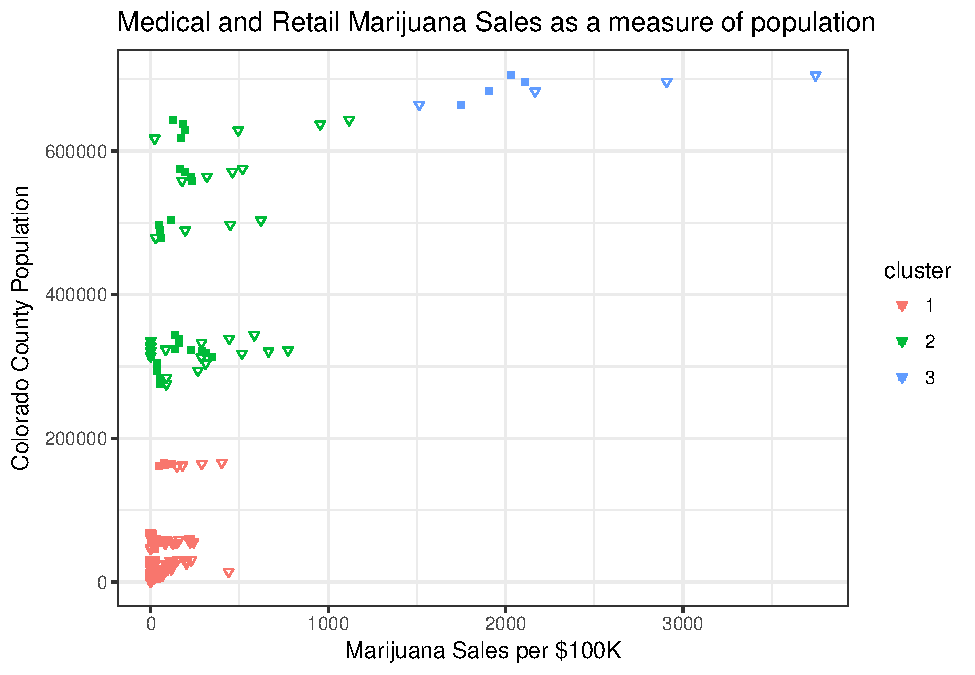
\includegraphics{01-Build_DS_and_EDA_files/figure-latex/unnamed-chunk-7-2.pdf}
The clusters didn't line up exactly as I expected but were grossly
right. I'll try drawing ellipses around the clusters.

\begin{Shaded}
\begin{Highlighting}[]
\KeywordTok{ggplot}\NormalTok{(}\DataTypeTok{data=}\NormalTok{CCMDs, }\KeywordTok{aes}\NormalTok{(}\DataTypeTok{x =}\NormalTok{ Population, }\DataTypeTok{color=}\NormalTok{cluster))}\OperatorTok{+}
\StringTok{  }\KeywordTok{geom_point}\NormalTok{(}\KeywordTok{aes}\NormalTok{(}\DataTypeTok{y =}\NormalTok{ Rec_Sales}\OperatorTok{/}\DecValTok{100000}\NormalTok{), }\DataTypeTok{show.legend =} \OtherTok{TRUE}\NormalTok{, }\DataTypeTok{size =} \FloatTok{1.25}\NormalTok{)}\OperatorTok{+}
\StringTok{  }\KeywordTok{stat_ellipse}\NormalTok{(}\KeywordTok{aes}\NormalTok{(}\DataTypeTok{y =}\NormalTok{ Rec_Sales}\OperatorTok{/}\DecValTok{100000}\NormalTok{))}\OperatorTok{+}
\StringTok{  }\KeywordTok{geom_smooth}\NormalTok{(}\KeywordTok{aes}\NormalTok{(}\DataTypeTok{y=}\NormalTok{Rec_Sales}\OperatorTok{/}\DecValTok{100000}\NormalTok{))}\OperatorTok{+}
\StringTok{  }\KeywordTok{geom_point}\NormalTok{(}\KeywordTok{aes}\NormalTok{(}\DataTypeTok{y =}\NormalTok{ Med_Sales}\OperatorTok{/}\DecValTok{100000}\NormalTok{), }\DataTypeTok{show.legend =} \OtherTok{TRUE}\NormalTok{, }\DataTypeTok{size =} \FloatTok{1.25}\NormalTok{)}\OperatorTok{+}
\StringTok{  }\KeywordTok{stat_ellipse}\NormalTok{(}\KeywordTok{aes}\NormalTok{(}\DataTypeTok{y =}\NormalTok{ Med_Sales}\OperatorTok{/}\DecValTok{100000}\NormalTok{))}\OperatorTok{+}
\StringTok{  }\KeywordTok{geom_smooth}\NormalTok{(}\KeywordTok{aes}\NormalTok{(}\DataTypeTok{y=}\NormalTok{Med_Sales}\OperatorTok{/}\DecValTok{100000}\NormalTok{))}\OperatorTok{+}
\StringTok{  }\KeywordTok{labs}\NormalTok{(}\DataTypeTok{title=}\StringTok{"Medical and Retail Marijuana Sales as a measure of population"}\NormalTok{, }\DataTypeTok{x=} \StringTok{"Colorado County Population"}\NormalTok{, }\DataTypeTok{y=} \StringTok{"Marijuana Sales per $100K"}\NormalTok{)}\OperatorTok{+}
\StringTok{  }\KeywordTok{theme_bw}\NormalTok{()}\OperatorTok{+}
\StringTok{  }\KeywordTok{coord_flip}\NormalTok{()}
\end{Highlighting}
\end{Shaded}

\begin{verbatim}
## `geom_smooth()` using method = 'loess'
\end{verbatim}

\begin{verbatim}
## Warning in simpleLoess(y, x, w, span, degree = degree, parametric =
## parametric, : span too small. fewer data values than degrees of freedom.
\end{verbatim}

\begin{verbatim}
## Warning in simpleLoess(y, x, w, span, degree = degree, parametric =
## parametric, : pseudoinverse used at 6.6451e+005
\end{verbatim}

\begin{verbatim}
## Warning in simpleLoess(y, x, w, span, degree = degree, parametric =
## parametric, : neighborhood radius 31837
\end{verbatim}

\begin{verbatim}
## Warning in simpleLoess(y, x, w, span, degree = degree, parametric =
## parametric, : reciprocal condition number 0
\end{verbatim}

\begin{verbatim}
## Warning in simpleLoess(y, x, w, span, degree = degree, parametric =
## parametric, : There are other near singularities as well. 5.1869e+008
\end{verbatim}

\begin{verbatim}
## Warning in predLoess(object$y, object$x, newx = if
## (is.null(newdata)) object$x else if (is.data.frame(newdata))
## as.matrix(model.frame(delete.response(terms(object)), : span too small.
## fewer data values than degrees of freedom.
\end{verbatim}

\begin{verbatim}
## Warning in predLoess(object$y, object$x, newx = if
## (is.null(newdata)) object$x else if (is.data.frame(newdata))
## as.matrix(model.frame(delete.response(terms(object)), : pseudoinverse used
## at 6.6451e+005
\end{verbatim}

\begin{verbatim}
## Warning in predLoess(object$y, object$x, newx = if
## (is.null(newdata)) object$x else if (is.data.frame(newdata))
## as.matrix(model.frame(delete.response(terms(object)), : neighborhood radius
## 31837
\end{verbatim}

\begin{verbatim}
## Warning in predLoess(object$y, object$x, newx = if
## (is.null(newdata)) object$x else if (is.data.frame(newdata))
## as.matrix(model.frame(delete.response(terms(object)), : reciprocal
## condition number 0
\end{verbatim}

\begin{verbatim}
## Warning in predLoess(object$y, object$x, newx = if
## (is.null(newdata)) object$x else if (is.data.frame(newdata))
## as.matrix(model.frame(delete.response(terms(object)), : There are other
## near singularities as well. 5.1869e+008
\end{verbatim}

\begin{verbatim}
## `geom_smooth()` using method = 'loess'
\end{verbatim}

\begin{verbatim}
## Warning in simpleLoess(y, x, w, span, degree = degree, parametric =
## parametric, : span too small. fewer data values than degrees of freedom.
\end{verbatim}

\begin{verbatim}
## Warning in simpleLoess(y, x, w, span, degree = degree, parametric =
## parametric, : pseudoinverse used at 6.6451e+005
\end{verbatim}

\begin{verbatim}
## Warning in simpleLoess(y, x, w, span, degree = degree, parametric =
## parametric, : neighborhood radius 31837
\end{verbatim}

\begin{verbatim}
## Warning in simpleLoess(y, x, w, span, degree = degree, parametric =
## parametric, : reciprocal condition number 0
\end{verbatim}

\begin{verbatim}
## Warning in simpleLoess(y, x, w, span, degree = degree, parametric =
## parametric, : There are other near singularities as well. 5.1869e+008
\end{verbatim}

\begin{verbatim}
## Warning in predLoess(object$y, object$x, newx = if
## (is.null(newdata)) object$x else if (is.data.frame(newdata))
## as.matrix(model.frame(delete.response(terms(object)), : span too small.
## fewer data values than degrees of freedom.
\end{verbatim}

\begin{verbatim}
## Warning in predLoess(object$y, object$x, newx = if
## (is.null(newdata)) object$x else if (is.data.frame(newdata))
## as.matrix(model.frame(delete.response(terms(object)), : pseudoinverse used
## at 6.6451e+005
\end{verbatim}

\begin{verbatim}
## Warning in predLoess(object$y, object$x, newx = if
## (is.null(newdata)) object$x else if (is.data.frame(newdata))
## as.matrix(model.frame(delete.response(terms(object)), : neighborhood radius
## 31837
\end{verbatim}

\begin{verbatim}
## Warning in predLoess(object$y, object$x, newx = if
## (is.null(newdata)) object$x else if (is.data.frame(newdata))
## as.matrix(model.frame(delete.response(terms(object)), : reciprocal
## condition number 0
\end{verbatim}

\begin{verbatim}
## Warning in predLoess(object$y, object$x, newx = if
## (is.null(newdata)) object$x else if (is.data.frame(newdata))
## as.matrix(model.frame(delete.response(terms(object)), : There are other
## near singularities as well. 5.1869e+008
\end{verbatim}

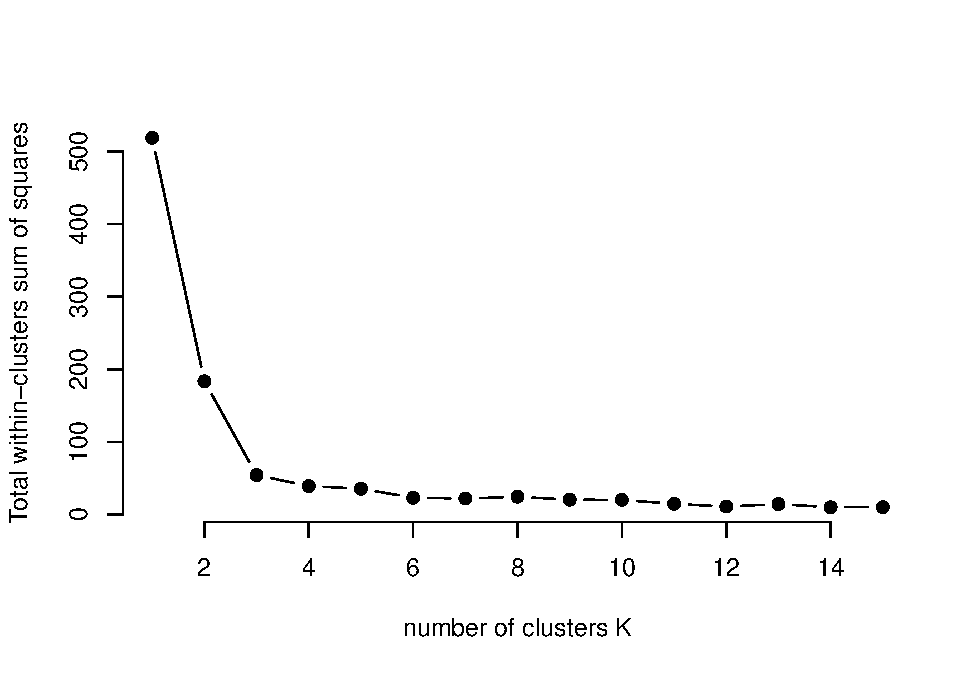
\includegraphics{01-Build_DS_and_EDA_files/figure-latex/unnamed-chunk-8-1.pdf}

\begin{Shaded}
\begin{Highlighting}[]
\KeywordTok{ggplot}\NormalTok{(}\DataTypeTok{data=}\NormalTok{CCMDs, }\KeywordTok{aes}\NormalTok{(}\DataTypeTok{x =}\NormalTok{ Population, }\DataTypeTok{color=}\NormalTok{cluster))}\OperatorTok{+}
\StringTok{  }\KeywordTok{geom_point}\NormalTok{(}\KeywordTok{aes}\NormalTok{(}\DataTypeTok{y =}\NormalTok{ Rec_Sales}\OperatorTok{/}\DecValTok{100000} \OperatorTok{+}\StringTok{ }\NormalTok{Med_Sales}\OperatorTok{/}\DecValTok{100000}\NormalTok{), }\DataTypeTok{show.legend =} \OtherTok{TRUE}\NormalTok{, }\DataTypeTok{size =} \FloatTok{1.25}\NormalTok{)}\OperatorTok{+}
\StringTok{  }\KeywordTok{stat_ellipse}\NormalTok{(}\KeywordTok{aes}\NormalTok{(}\DataTypeTok{y =}\NormalTok{ Rec_Sales}\OperatorTok{/}\DecValTok{100000} \OperatorTok{+}\StringTok{ }\NormalTok{Med_Sales}\OperatorTok{/}\DecValTok{100000}\NormalTok{))}\OperatorTok{+}
\StringTok{  }\KeywordTok{theme_bw}\NormalTok{()}\OperatorTok{+}
\StringTok{  }\KeywordTok{coord_flip}\NormalTok{()}
\end{Highlighting}
\end{Shaded}

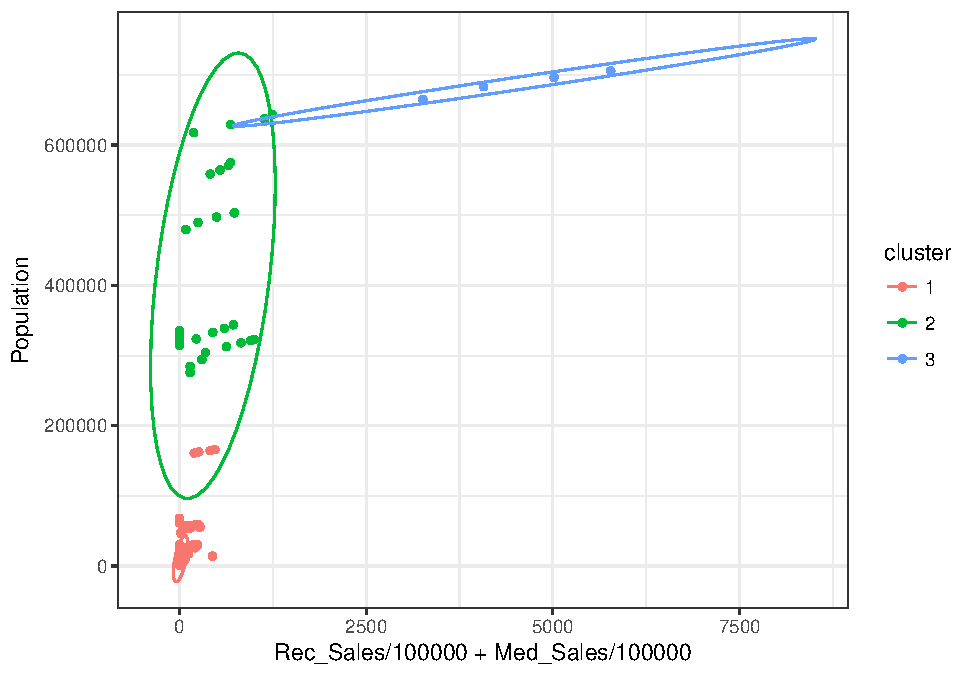
\includegraphics{01-Build_DS_and_EDA_files/figure-latex/unnamed-chunk-8-2.pdf}
A lot of warnings that I need to disect. The cluster smoothing pattern
goes beyond -1 (I think) due to using the mean instead of the median. I
think I can fix that. Also, I think a next step should be try the same
exercise as above with Principal Component Analysis (PCA). I'm
interested in the eigenvector values\ldots{}

ref: \url{http://rpubs.com/sinhrks/plot_pca}

spare or inwork stuff\ldots{}

ggplot(data=CCMDs, aes(x = Population))+ geom\_point(aes(y =
Rec\_Sales/100000), color=``green'', show.legend = TRUE, size = 1.25)+
labs(title=``Retail Marijuana Sales as a measure of population'', x=
``Colorado County Population'', y= ``Marijuana Sales per \$100K'')+
theme\_bw()+ coord\_flip()

ggplot(data=CCMDs, aes(x = Population))+ geom\_point(aes(y =
Med\_Sales/100000), color=``red'', show.legend = TRUE, size = 1.25)+
labs(title=``Medical Marijuana Sales as a measure of population'', x=
``Colorado County Population'', y= ``Marijuana Sales per \$100K'')+
theme\_bw()+ coord\_flip()

ggplot(data=CCMDs, mapping=aes(x=Year))+
geom\_col(mapping=aes(y=Rec\_Sales/100000), position=position\_dodge(),
fill=``green'')+ geom\_col(mapping=aes(y=Med\_Sales/100000),
position=position\_dodge() , fill=``red'')+ labs(title=``Colorado
Medical and Retail Marijuana Sales 2014-2018'', x= ``Years of
Recreational Legalization'', y= ``Sales per \$100K'')+ theme\_bw()

ggplot(data=CCMDs, aes(x=as.factor(CCMDs\$County)))+
geom\_boxplot(aes(y=Rec\_Sales), color=``green'')+
geom\_boxplot(aes(y=Med\_Sales), color=``red'')+ labs(title=``Colorado
Retail and Medical Marijuana Sales since 2014'', x= ``Colorado County'',
y= ``Sales'')+ theme\_bw()+ theme(axis.text.x = element\_text(angle =
90, hjust = 1))

ggplot(data=CCMDs, mapping=aes(x=Year))+ geom\_jitter(aes(y=Rec\_Sales),
color=``green'')+ geom\_jitter(aes(y=Med\_Sales), color=``red'')+
labs(title=``Colorado Medical and Retail Marijuana Sales 2014-2018'', x=
``Years of Recreational Legalization'', y= ``Sales per \$100K'')+
theme\_bw()

CCMDs\_pop \textless{}- CCMDs{[}, c(1,2,7){]}
CCMDs\_pop\(County <- as.factor(CCMDs_pop\)County) CCMDs\_pop
\textless{}- CCMDs\_pop{[}order(CCMDs\_pop\$Population),{]}

str(CCMDs\_pop)

\#CCMDs\_pop \textless{}- CCMDs\_pop{[}order(CCMDs\_pop\$Population),{]}

View(CCMDs\_pop)

\#ggplot(data=CCMDs, mapping=aes(x=Year, y=Population, group=Region))+
\# geom\_line(color=``red'')+ \# geom\_point(color=``red'')+ \#
scale\_y\_continuous(limits =
c(min(CCMDs\(Population), max(CCMDs\)Population)))+ \#
geom\_label\_repel(aes(label = Population), nudge\_x = 1)+ \#
labs(title=``Colorado Estimated Population Growth since 2010 Census'')+
\# theme\_bw()

\#CCMDs\_pop \textless{}- data.frame(order(CCMDs\_pop\$Population))

ggplot(data=CCMDs\_pop, mapping=aes(x=County, y=Population))+
geom\_bar(stat=``identity'', position=``dodge'', fill=``blue'')+
labs(title=``Colorado Population by County'', x= ``County'', y=
``Population'')+ theme\_bw()+ theme(axis.text.x = element\_text(angle =
90))

ggplot(data=CCMDs\_pop, aes(x=as.factor(CCMDs\_pop\$County)))+
geom\_boxplot(aes(y=Population), color=``blue'')+ labs(title=``Colorado
Population by County'', x= ``County'', y= ``Population'')+ theme\_bw()+
theme(axis.text.x = element\_text(angle = 90))

```

\#corrplot the value features \#m \textless{}- cor(CCMDs{[}, c(8:14){]},
use = ``complete.obs'', method = ``spearman'') \#require(``corrplot'')
\#corrplot(m, type = ``upper'', order = ``hclust'', tl.srt = 45)


\end{document}
